\documentclass[border=3mm]{standalone}

\usepackage{tikz}

\begin{document}
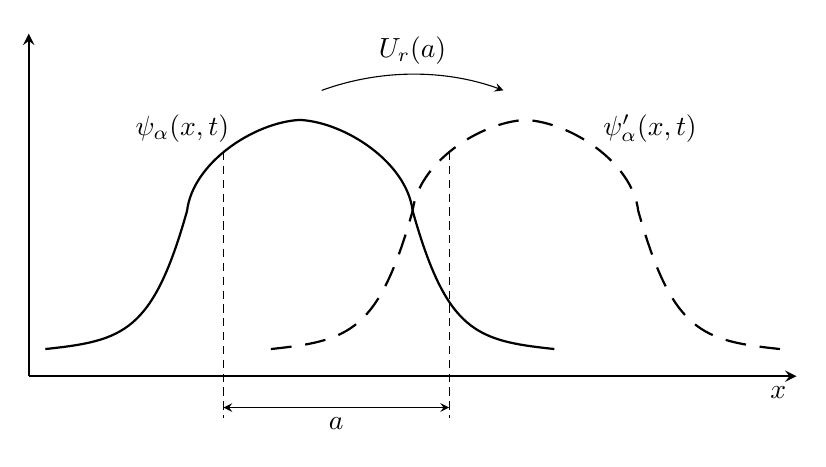
\begin{tikzpicture}[scale=0.75]
\draw[-stealth,thick] (0,0) -- (0,5.8);
\draw[-stealth,thick] (0,0) -- (13,0) node[below left] {$x$};
\draw[thick] (0.28,0.46) .. controls (1.6,0.6) and (2.1,0.74) .. (2.68,2.8) .. controls (2.78,3.62) and (3.82,4.3) ..  coordinate[pos=0.46](a) (4.59,4.34) .. controls (5.36,4.3) and (6.4,3.62) .. (6.5,2.8) .. controls (7.08,0.74) and (7.58,0.6) .. (8.9,0.46);
\draw[densely dashed] (a) --++(0,-4.5cm) coordinate (1);
\draw[dash pattern=on 7.5pt off 5pt,thick] (4.1,0.46) .. controls (5.42,0.6) and (5.92,0.74) .. (6.5,2.8) .. controls (6.6,3.62) and (7.64,4.3) ..  coordinate[pos=0.46](b) (8.41,4.34) .. controls (9.18,4.3) and (10.22,3.62) .. (10.32,2.8) .. controls (10.9,0.74) and (11.4,0.6) .. (12.72,0.46);
\draw[densely dashed] (b) --++(0,-4.5cm) coordinate (2);
\draw[-stealth] (4.96,4.84) arc (110:70:4.5) node[midway,above] {$U_{r}(a)$};
\draw[stealth-stealth] ([yshift=5pt]1) -- ([yshift=5pt]2) node[midway,below] {$a$};
\node at (2.6,4.2) {$\psi_{\alpha}(x,t)$};
\node at (10.52,4.2) {$\psi'_{\alpha}(x,t)$};
\end{tikzpicture}
\end{document}